\documentclass[]{apuntes_itsv}
\usepackage{listings}
\usepackage{tikz}
\usetikzlibrary{shapes.geometric, arrows.meta, positioning, calc, babel}
\usepackage[backend=bibtex, style=alphabetic, sorting=ynt]{biblatex}
\addbibresource{fuentes.bib}

\definecolor{codegreen}{rgb}{0,0.6,0}
\definecolor{codegray}{rgb}{0.5,0.5,0.5}
\definecolor{codepurple}{rgb}{0.58,0,0.82}
\definecolor{backcolour}{rgb}{0.96,0.96,0.96}

\setlength{\parskip}{5pt}

\lstdefinestyle{pystyle}{
    backgroundcolor=\color{backcolour},
    commentstyle=\color{codegreen},
    keywordstyle=\color{magenta},
    numberstyle=\tiny\color{codegray},
    stringstyle=\color{codepurple},
    basicstyle=\ttfamily\small,
    breakatwhitespace=false,
    breaklines=true,
    captionpos=b,
    keepspaces=true,
    numbers=left,
    numbersep=5pt,
    showspaces=false,
    showstringspaces=false,
    showtabs=false,
    tabsize=4,
    frame=single,
    language=Python,
    extendedchars=true,
    literate=
    {á}{{\'a}}1
    {é}{{\'e}}1
    {í}{{\'i}}1
    {ó}{{\'o}}1
    {ú}{{\'u}}1
    {Á}{{\'A}}1
    {É}{{\'E}}1
    {Í}{{\'I}}1
    {Ó}{{\'O}}1
    {Ú}{{\'U}}1
    {ñ}{{\~n}}1
    {Ñ}{{\~N}}1
}
\lstset{style=pystyle}

% Datos del documento
\titulo{Programación Orientada a Objetos}
\catedra{Programación I}
\curso{4to año C}
\docentes{Cortesini Pérez Luciano Tomás, Bisio Facundo} % TODO: Agregar nombre completo de facu bisio
\fecha{\today}

\begin{document}

\maketitle
\tableofcontents

% Capítulos
\chapter{Introducción}

Todos tenemos una idea intuitiva de qué es un objeto: es una cosa que podemos percibir, manipular y con la que podemos interactuar.

Por ejemplo, pensemos en un fibrón de pizarra. Podemos describir este objeto a partir de sus características: tiene una
determinada masa, color, forma, tamaño, etc. Estas características nos permiten describir el estado del objeto.

Pero un fibrón no solamente tiene características. También podemos realizar determinadas acciones con él. Podemos, por
ejemplo, escribir o dibujar sobre una pizarra utilizando el fibrón. También podemos realizar acciones sobre el propio
objeto, como ponerle o quitarle la tapa.

Un fibrón, además, no necesariamente tiene que ser considerado como un objeto aislado. Podemos observar que está
formado por distintas partes: un cuerpo, una tapa, una punta, etc. Cada una de estas partes podría, a su vez, ser
considerada como un objeto.

También podemos observar que un fibrón pertenece a una categoría más general de objetos: los útiles de escritura. Dentro
de esta categoría podemos encontrar lápices, lapiceras, marcadores, crayones, etc. Estos objetos comparten determinadas
características y comportamientos, aunque cada uno tenga sus particularidades.

Esta forma de pensar los objetos —qué características tienen, qué pueden hacer, cómo se relacionan con otros objetos y
qué tienen en común— es precisamente la base de la Programación Orientada a Objetos.

La definición de un objeto en el desarrollo de software no es muy diferente. Los objetos de software pueden no ser cosas
tangibles que podamos agarrar, percibir o tocar, pero son \textbf{modelos} de algo que puede realizar determinadas acciones y sobre el cual
se pueden realizar determinadas acciones. Formalmente, un objeto es una \textbf{colección de datos y comportamientos asociados}.

Veremos a lo largo de este apunte que los conceptos que utilizamos para describir el fibrón tienen su equivalente en POO.

\section{De la Programación Estructurada a la POO}
Hasta el momento, siempre tuvimos por un lado nuestros datos almacenados en variables, como enteros, listas, diccionarios, etc.
Y por otro lado, los procedimientos, descriptos en funciones, que reciben, procesan y devuelven un resultado. Esta forma de estructurar
el programa es conocido como programación estucturada.

Sin embargo, a medida que los problemas de software aumentan en complejidad, la separación entre
datos y funciones dificulta el mantenimiento y la escalabilidad del código.
La \textit{Programación Orientada a Objetos} (POO) propone una forma distinta de organizar y estructurar
el código: agrupar los datos y las acciones que los manipulan dentro de una misma entidad llamada \textit{objeto}.

\begin{figure}[!ht]
  \centering
  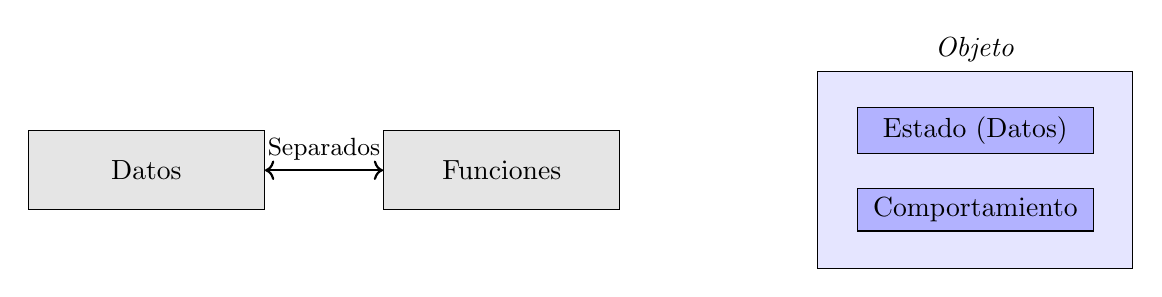
\begin{tikzpicture}[node distance=2cm, auto]
    % Estructurada
    \node [draw, rectangle, fill=gray!20, minimum width=3cm, minimum height=1cm] (datos) {Datos};
    \node [draw, rectangle, fill=gray!20, minimum width=3cm, minimum height=1cm, right=1.5cm of datos] (func) {Funciones};
    \draw[<->, thick] (datos) -- node[above] {\small Separados} (func);
    
    % POO
    \node [draw, rectangle, fill=blue!10, minimum width=4cm, minimum height=2.5cm, right=2.5cm of func] (objeto) {};
    \node [above] at (objeto.north) {\textit{Objeto}};
    \node [draw, rectangle, fill=blue!30, minimum width=3cm, baseline] at ($(objeto.center)+(0,0.5)$) {Estado (Datos)};
    \node [draw, rectangle, fill=blue!30, minimum width=3cm, baseline] at ($(objeto.center)+(0,-0.5)$) {Comportamiento};
  \end{tikzpicture}
  \caption{Comparación entre Programación Estructurada y Programación Orientada a Objetos.}
  \label{fig:estructurada_vs_poo}
\end{figure}

Como se ilustra en la \fig{fig:estructurada_vs_poo}, la POO permite integrar el estado y el comportamiento
en un bloque cohesivo, facilitando el modelado de sistemas complejos.

\section{¿Qué es un Objeto?}
En el mundo real, un objeto es cualquier entidad física o abstracta que posee características y realiza acciones.
Por ejemplo, un fibrón de pizarra tiene características como color, marca y masa, y realiza acciones como
escribir o ser borrado. Del mismo modo, un automóvil tiene un modelo, patente, kilometraje y color, y acciones
como acelerar, frenar o doblar.

En programación, un \textit{objeto} es un modelo conceptual que almacena información y define comportamientos
asociados. Todo objeto se compone de dos elementos fundamentales:

\begin{itemize}[leftmargin=*]
  \item \textit{Atributos}: representan el estado o las características del objeto (por ejemplo, el saldo de una cuenta bancaria).
  \item \textit{Métodos}: representan las acciones o procedimientos que el objeto puede ejecutar (por ejemplo, depositar o retirar dinero).
\end{itemize}

\section{Clases y Objetos: Moldes e Instancias}
Para crear objetos en un programa, primero debemos definir su estructura mediante una \textit{clase}.
Una clase funciona como un plano o plantilla arquitectónica que especifica qué atributos y métodos
tendrán los objetos construidos a partir de ella.

Un \textit{objeto} es una \textit{instancia} concreta de una clase. Aunque dos personas tengan un automóvil
del mismo modelo (construidos con el mismo plano), cada automóvil es un objeto independiente con su propia
patente, kilometraje acumulado y estado de desgaste.

\begin{figure}[!ht]
  \centering
  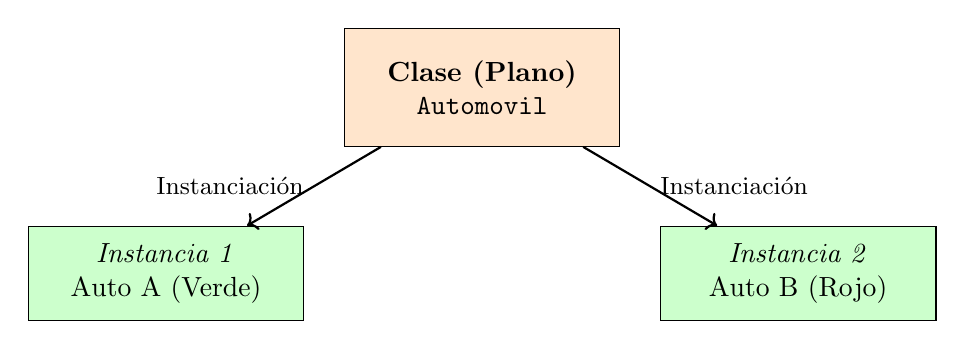
\begin{tikzpicture}[node distance=2.5cm]
    \node [draw, rectangle, fill=orange!20, minimum width=3.5cm, minimum height=1.5cm, align=center] (clase) 
      {\textbf{Clase (Plano)}\\ \texttt{Automovil}};
    
    \node [draw, rectangle, fill=green!20, minimum width=3.5cm, minimum height=1.2cm, align=center, below left=1cm and 0.5cm of clase] (obj1) 
      {\textit{Instancia 1}\\ Auto A (Verde)};
    
    \node [draw, rectangle, fill=green!20, minimum width=3.5cm, minimum height=1.2cm, align=center, below right=1cm and 0.5cm of clase] (obj2) 
      {\textit{Instancia 2}\\ Auto B (Rojo)};
    
    \draw[->, thick] (clase) -- node[left] {\small Instanciación} (obj1);
    \draw[->, thick] (clase) -- node[right] {\small Instanciación} (obj2);
  \end{tikzpicture}
  \caption{Relación entre una Clase (plantilla) y sus Instancias (objetos reales).}
  \label{fig:clase_objeto}
\end{figure}

Como se observa en la \fig{fig:clase_objeto}, una única definición de clase permite instanciar múltiples objetos
con valores de atributos independientes en memoria.

\chapter{Clases, Objetos y Atributos de Instancia}

\section{Definición de una Clase en Python}
Para declarar una clase en Python se utiliza la palabra reservada \texttt{class}, seguida del nombre de la clase
(escrito convencionalmente en formato \textit{CamelCase}) y dos puntos.
Si deseamos definir una clase vacía sin atributos ni métodos iniciales, empleamos la sentencia \texttt{pass} como
marcador de posición sintáctico.

\begin{lstlisting}[caption={Definición de una clase vacía y su instanciación.}, label={list:clase_vacia}]
class Vehicle:
    """Clase base que representa un vehiculo generico."""
    pass

# Inspeccion del objeto clase
print(Vehicle)
\end{lstlisting}

En el \sect{list:clase_vacia} se observa el uso de un \textit{docstring} (cadena literal encerrada entre tres comillas),
el cual permite documentar la función o propósito de la clase directamente en el código fuente.

\section{El Constructor \texttt{\_\_init\_\_} y el Parámetro \texttt{self}}
Cuando se crea una nueva instancia de una clase, Python ejecuta automáticamente un método especial de inicialización
llamado \texttt{\_\_init\_\_}. Este método actúa como el constructor de la clase, reservando espacio y asignando los
valores iniciales a los atributos del objeto.

El primer parámetro de todo método de instancia en Python debe ser obligatoriamente \texttt{self}. El parámetro
\texttt{self} es una referencia explícita a la instancia concreta sobre la cual se está ejecutando el método.

\begin{lstlisting}[caption={Uso del constructor y asignación de atributos de instancia.}, label={list:init_atributos}]
class Vehicle:
    """Representa un vehiculo con velocidad maxima y kilometraje."""
    
    def __init__(self, name, max_speed, mileage):
        self.name = name
        self.max_speed = max_speed
        self.mileage = mileage

# Instanciacion de objetos independientes
v1 = Vehicle("Tesla Model S", 250, 18)
v2 = Vehicle("Toyota Corolla", 180, 45000)

print(f"Vehiculo 1: {v1.name}, Maxima: {v1.max_speed} km/h")
print(f"Vehiculo 2: {v2.name}, Maxima: {v2.max_speed} km/h")
\end{lstlisting}

Al ejecutar la línea \texttt{v1 = Vehicle("Tesla Model S", 250, 18)}, Python invoca internamente a
\texttt{Vehicle.\_\_init\_\_(v1, "Tesla Model S", 250, 18)}. La notación de punto (\texttt{v1.name})
permite acceder a los atributos específicos almacenados en esa instancia.

\section{Métodos de Instancia}
Los métodos de instancia son funciones definidas dentro de una clase que operan sobre los datos almacenados
en los atributos de la instancia actual. A través del parámetro \texttt{self}, los métodos pueden leer o modificar
el estado interno del objeto.

\subsection{Cálculos Derivados a partir de Atributos}
Un patrón habitual en POO es la creación de métodos que calculan nueva información utilizando los atributos
almacenados en la instancia.

\begin{lstlisting}[caption={Clase Rectangle con métodos de cálculo geométrico.}, label={list:rectangle}]
class Rectangle:
    def __init__(self, length, width):
        self.length = length
        self.width = width

    def area(self):
        """Calcula el area del rectangulo."""
        return self.length * self.width

    def perimeter(self):
        """Calcula el perimetro del rectangulo."""
        return 2 * (self.length + self.width)

rect = Rectangle(10, 4)
print(f"Area: {rect.area()}")
print(f"Perimetro: {rect.perimeter()}")
\end{lstlisting}

Al llamar a \texttt{rect.area()}, no es necesario pasar el argumento \texttt{self} explícitamente, ya que Python
asocia automáticamente el objeto \texttt{rect} invocante.

\subsection{Validación de Datos y Reglas de Negocio}
Los métodos también se utilizan para imponer restricciones y validar las operaciones sobre el estado interno.
Un ejemplo clásico es la gestión de cuentas bancarias con protección contra sobregiros.

\begin{lstlisting}[caption={Clase BankAccount con validación de saldo.}, label={list:bank_account}]
class BankAccount:
    def __init__(self, owner, balance=0.0):
        self.owner = owner
        self.balance = balance

    def deposit(self, amount):
        if amount > 0:
            self.balance += amount
            print(f"Deposito de {amount} exitoso. Saldo actual: {self.balance}")
        else:
            print("El monto a depositar debe ser positivo.")

    def withdraw(self, amount):
        if amount > self.balance:
            print("Fondos insuficientes. Operacion cancelada.")
        elif amount <= 0:
            print("Monto de retiro invalido.")
        else:
            self.balance -= amount
            print(f"Retiro de {amount} exitoso. Saldo restante: {self.balance}")

cuenta = BankAccount("Juan", 1000)
cuenta.deposit(500)
cuenta.withdraw(2000)  # Muestra mensaje de fondos insuficientes
\end{lstlisting}

\subsection{Gestión del Estado Interno y Alternancia de Estados}
Los objetos pueden cambiar de estado mediante métodos dedicados a modificar variables booleanas o banderas internas.

\begin{lstlisting}[caption={Clase Light con métodos para alternar su estado.}, label={list:light}]
class Light:
    def __init__(self):
        self.is_on = False

    def turn_on(self):
        self.is_on = True

    def turn_off(self):
        self.is_on = False

    def toggle(self):
        self.is_on = not self.is_on
\end{lstlisting}

\section{Atributos con Estructuras de Datos Complejas}
Los atributos de una instancia no se limitan a tipos primarios (enteros, cadenas, flotantes); también pueden
almacenar colecciones completas como listas, diccionarios o conjuntos.

\begin{lstlisting}[caption={Clase Student almacenando una lista de notas.}, label={list:student}]
class Student:
    def __init__(self, name, marks):
        self.name = name
        self.marks = marks  # Lista de numeros flotantes o enteros

    def average(self):
        if not self.marks:
            return 0.0
        return sum(self.marks) / len(self.marks)

s1 = Student("Alice", [85, 90, 78, 92, 88])
print(f"Promedio de {s1.name}: {s1.average():.2f}")
\end{lstlisting}

\chapter{Atributos de Clase y Métodos Especiales}

\section{Atributos de Clase vs Atributos de Instancia}
En Python existen dos tipos de atributos según su ámbito de pertenencia:

\begin{itemize}[leftmargin=*]
  \item \textit{Atributos de instancia}: pertenecen a un objeto específico y son inicializados habitualmente
    dentro del método \texttt{\_\_init\_\_} mediante \texttt{self.atributo}. Cada instancia mantiene su propia copia.
  \item \textit{Atributos de clase}: se definen directamente en el cuerpo de la clase (fuera de cualquier método)
    y son compartidos por todas las instancias creadas a partir de dicha clase.
\end{itemize}

\begin{lstlisting}[caption={Diferencia entre atributos de clase y de instancia.}, label={list:atributos_clase}]
class Student:
    # Atributo de clase (compartido por todos los estudiantes)
    school_name = "Instituto Técnico Salesiano Villada"

    def __init__(self, name, age):
        # Atributos de instancia (unicos para cada objeto)
        self.name = name
        self.age = age

e1 = Student("Lucas", 16)
e2 = Student("Sofia", 16)

print(e1.school_name)  # Muestra el valor de clase
print(e2.school_name)

# Modificacion mediante el nombre de la clase
Student.school_name = "ITSV Cordoba"
print(e1.school_name)  # Refleja el cambio en todas las instancias
\end{lstlisting}

Si se modifica un atributo de clase utilizando la referencia del nombre de la clase (\texttt{Student.school\_name}),
el cambio impacta en todas las instancias que no hayan sobrescrito dicho atributo a nivel de instancia.

\section{Métodos Especiales (Dunder Methods)}
Los métodos especiales, conocidos popularmente como \textit{dunder methods} (por la abreviatura de \textit{double underscore}),
son métodos cuyo nombre inicia y finaliza con dos guiones bajos, como por ejemplo \texttt{\_\_init\_\_}.
Python los utiliza para sobrecargar operadores y personalizar comportamientos integrados del lenguaje.

\subsection{Representación como Cadena: \texttt{\_\_str\_\_} y \texttt{\_\_repr\_\_}}
Cuando se imprime un objeto mediante \texttt{print()} o se convierte a cadena con \texttt{str()}, Python busca
el método \texttt{\_\_str\_\_}. Cuando se inspecciona en la consola interactiva o dentro de colecciones, se utiliza \texttt{\_\_repr\_\_}.

\begin{itemize}[leftmargin=*]
  \item \texttt{\_\_str\_\_}: pensado para presentar una salida amigable y legible para el usuario final.
  \item \texttt{\_\_repr\_\_}: pensado para proporcionar una representación inequívoca, útil para desarrolladores durante el proceso de depuración.
\end{itemize}

\begin{lstlisting}[caption={Implementación de \texttt{\_\_str\_\_} y \texttt{\_\_repr\_\_}.}, label={list:str_repr}]
class Book:
    def __init__(self, title, author):
        self.title = title
        self.author = author

    def __str__(self):
        return f"'{self.title}' escrito por {self.author}"

    def __repr__(self):
        return f"Book(title='{self.title}', author='{self.author}')"

libro = Book("Python Crash Course", "Eric Matthes")
print(str(libro))   # Invoca __str__
print(repr(libro))  # Invoca __repr__
\end{lstlisting}

\subsection{Sobrecarga de Operadores Aritméticos: \texttt{\_\_add\_\_}}
La sobrecarga de operadores permite definir cómo se comportarán los operadores matemáticos estándar
(como \texttt{+}, \texttt{-}, \texttt{*}) cuando se apliquen sobre objetos de nuestras propias clases.

\begin{lstlisting}[caption={Sobrecarga del operador suma mediante \texttt{\_\_add\_\_}.}, label={list:vector_add}]
class Vector2D:
    def __init__(self, x, y):
        self.x = x
        self.y = y

    def __add__(self, other):
        if isinstance(other, Vector2D):
            return Vector2D(self.x + other.x, self.y + other.y)
        return NotImplemented

    def __str__(self):
        return f"Vector({self.x}, {self.y})"

v1 = Vector2D(2, 4)
v2 = Vector2D(3, 1)
v3 = v1 + v2  # Invoca v1.__add__(v2)
print(v3)     # Salida: Vector(5, 5)
\end{lstlisting}

\subsection{Métodos Especiales \texttt{\_\_len\_\_} y \texttt{\_\_call\_\_}}
El método \texttt{\_\_len\_\_} permite a una clase responder a la función integrada \texttt{len()}.

\begin{lstlisting}[caption={Uso de \texttt{\_\_len\_\_} para calcular la cantidad de elementos.}, label={list:cart_len}]
class ShoppingCart:
    def __init__(self):
        self.items = []

    def add_item(self, item):
        self.items.append(item)

    def __len__(self):
        return len(self.items)

cart = ShoppingCart()
cart.add_item("Manzana")
cart.add_item("Pan")
print(f"Cantidad de productos: {len(cart)}")
\end{lstlisting}

Por otro lado, el método \texttt{\_\_call\_\_} permite que una instancia de una clase sea invocada como si fuera una función.

\begin{lstlisting}[caption={Instancia invocable con \texttt{\_\_call\_\_}.}, label={list:call_method}]
class Multiplier:
    def __init__(self, factor):
        self.factor = factor

    def __call__(self, x):
        return x * self.factor

duplicar = Multiplier(2)
print(duplicar(5))  # Retorna 10
\end{lstlisting}

\chapter{Herencia y Polimorfismo}

\section{Herencia}
La \textit{herencia} es un mecanismo fundamental de la POO que permite crear nuevas clases basadas en clases existentes.
La clase original se denomina \textit{superclase} o \textit{clase padre}, mientras que la nueva clase se llama
\textit{subclase} o \textit{clase hija}.

La subclase hereda automáticamente todos los atributos y métodos de la superclase, lo que fomenta la reutilización de código
y permite establecer jerarquías conceptuales del tipo \textit{``es-un''} (por ejemplo, un colectivo \textit{es un} vehículo).

\begin{figure}[!ht]
  \centering
  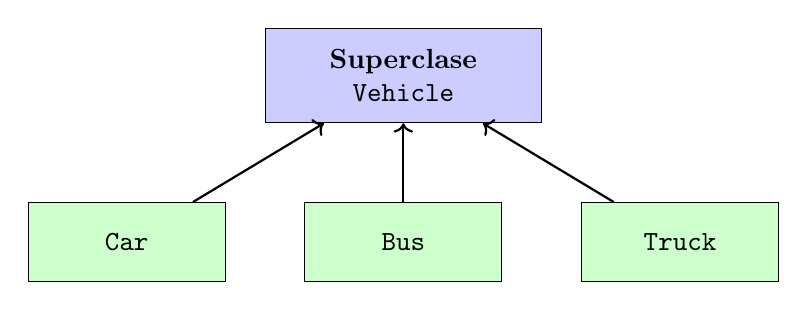
\begin{tikzpicture}[node distance=1.5cm, align=center]
    \node [draw, rectangle, fill=blue!20, minimum width=3.5cm, minimum height=1.2cm] (padre) 
      {\textbf{Superclase}\\ \texttt{Vehicle}};
    
    \node [draw, rectangle, fill=green!20, minimum width=2.5cm, minimum height=1cm, below left=1cm and 0.5cm of padre] (hijo1) 
      {\texttt{Car}};
    
    \node [draw, rectangle, fill=green!20, minimum width=2.5cm, minimum height=1cm, below=1cm of padre] (hijo2) 
      {\texttt{Bus}};
    
    \node [draw, rectangle, fill=green!20, minimum width=2.5cm, minimum height=1cm, below right=1cm and 0.5cm of padre] (hijo3) 
      {\texttt{Truck}};
    
    \draw[<-, thick] (padre) -- (hijo1);
    \draw[<-, thick] (padre) -- (hijo2);
    \draw[<-, thick] (padre) -- (hijo3);
  \end{tikzpicture}
  \caption{Jerarquía de herencia a partir de la superclase Vehicle.}
  \label{fig:herencia_vehiculos}
\end{figure}

\begin{lstlisting}[caption={Sintaxis básica de herencia en Python.}, label={list:herencia_basica}]
class Vehicle:
    def __init__(self, name, max_speed):
        self.name = name
        self.max_speed = max_speed

    def display_info(self):
        print(f"Vehiculo: {self.name}, Velocidad Maxima: {self.max_speed} km/h")

# Bus hereda de Vehicle
class Bus(Vehicle):
    pass

b = Bus("Mercedes Benz", 120)
b.display_info()  # Metodo heredado de Vehicle
\end{lstlisting}

\section{Sobrescritura de Métodos y Uso de \texttt{super()}}
En muchas situaciones, una subclase necesita adaptar o extender el comportamiento de un método heredado.
Este proceso se denomina \textit{sobrescritura de métodos} (\textit{method overriding}).

Para reutilizar la lógica de la superclase en lugar de reescribirla por completo, Python proporciona la función \texttt{super()}.

\begin{lstlisting}[caption={Uso de \texttt{super()} para extender el constructor y métodos.}, label={list:super_ejemplo}]
class Vehicle:
    def __init__(self, name, max_speed, mileage):
        self.name = name
        self.max_speed = max_speed
        self.mileage = mileage

    def fare(self):
        return self.mileage * 10

class Bus(Vehicle):
    def __init__(self, name, max_speed, mileage, capacity=50):
        # Llama al constructor de la superclase Vehicle
        super().__init__(name, max_speed, mileage)
        self.capacity = capacity

    def fare(self):
        # Sobrescribe el metodo agregando un 10% de mantenimiento
        base_fare = super().fare()
        total_fare = base_fare + (base_fare * 0.10)
        return total_fare

bus = Bus("Escolar", 90, 100, 40)
print(f"Tarifa del colectivo: ${bus.fare()}")
\end{lstlisting}

\section{Inspección de Tipos y Jerarquías}
Python dispone de funciones integradas para consultar la pertenencia de un objeto a una clase o jerarquía:

\begin{itemize}[leftmargin=*]
  \item \texttt{type(obj)}: retorna la clase exacta a la cual pertenece un objeto.
  \item \texttt{isinstance(obj, Clase)}: comprueba si un objeto es una instancia de la clase especificada o de una subclase derivada de ella.
  \item \texttt{issubclass(Subclase, Superclase)}: verifica si una clase hereda de otra superclase.
\end{itemize}

\begin{lstlisting}[caption={Uso de \texttt{isinstance()} e \texttt{issubclass()}.}, label={list:inspeccion_tipos}]
b = Bus("Urbano", 80, 50)

print(type(b))                       # <class '__main__.Bus'>
print(isinstance(b, Bus))           # True
print(isinstance(b, Vehicle))       # True (por herencia)
print(issubclass(Bus, Vehicle))     # True
\end{lstlisting}

\section{Polimorfismo}
El \textit{polimorfismo} es la capacidad que poseen distintos objetos de responder al mismo mensaje o llamada
de método, ejecutando cada uno su propia implementación específica.

En Python, el polimorfismo se aplica frecuentemente mediante el principio de \textit{Duck Typing} (``Si camina como
un pato y suena como un pato, entonces es un pato''). Esto significa que a una función no le importa la clase exacta
del objeto recibido, sino que este responda a los métodos invocados.

\begin{lstlisting}[caption={Polimorfismo con jerarquía de animales.}, label={list:polimorfismo_animales}]
class Dog:
    def speak(self):
        return "Guau!"

class Cat:
    def speak(self):
        return "Miau!"

def hacer_sonar(animal):
    # Invoca speak() de forma polimorfica sin importar el tipo exacto
    print(animal.speak())

mascotas = [Dog(), Cat()]
for m in mascotas:
    hacer_sonar(m)
\end{lstlisting}

Un ejemplo aplicado al cálculo de salarios en un sistema de recursos humanos ilustra el valor del polimorfismo:

\begin{lstlisting}[caption={Polimorfismo aplicado al cálculo de salarios.}, label={list:polimorfismo_empleados}]
class Employee:
    def __init__(self, name):
        self.name = name

    def calculate_salary(self):
        raise NotImplementedError("Las subclases deben implementar este metodo.")

class FullTimeEmployee(Employee):
    def __init__(self, name, monthly_salary):
        super().__init__(name)
        self.monthly_salary = monthly_salary

    def calculate_salary(self):
        return self.monthly_salary

class PartTimeEmployee(Employee):
    def __init__(self, name, hours_worked, hourly_rate):
        super().__init__(name)
        self.hours_worked = hours_worked
        self.hourly_rate = hourly_rate

    def calculate_salary(self):
        return self.hours_worked * self.hourly_rate

empleados = [
    FullTimeEmployee("Carlos", 350000),
    PartTimeEmployee("Ana", 80, 2500)
]

for e in empleados:
    print(f"Empleado: {e.name}, Salario: ${e.calculate_salary()}")
\end{lstlisting}

\chapter{Encapsulamiento y Composición}

\section{Encapsulamiento y Ocultamiento de Información}
El \textit{encapsulamiento} es el principio de la POO que consiste en ocultar los detalles internos de implementación
de un objeto y restringir el acceso directo a sus atributos desde el exterior del código de la clase.
Esto evita que los datos internos sean modificados de forma arbitraria o inconsistente.

A diferencia de lenguajes como C++ o Java, Python no posee palabras clave como \texttt{private} o \texttt{protected}
a nivel de compilador, sino que emplea convenciones de nombres para indicar la privacidad de los miembros.

\subsection{Atributos Protegidos (\texttt{\_atributo})}
Un atributo cuyo nombre comienza con un único guion bajo (por ejemplo, \texttt{\_balance}) indica convencionalmente
que es un miembro protegido. Aunque Python permite acceder a él desde el exterior, la regla indica que solo debería
ser utilizado internamente por la clase y sus subclases.

\subsection{Atributos Privados (\texttt{\_\_atributo}) y Name Mangling}
Cuando un atributo comienza con dos guiones bajos (por ejemplo, \texttt{\_\_balance}), Python activa un mecanismo
llamado \textit{Name Mangling} (modificación de nombres). El interprete transforma internamente el nombre del atributo
agregando el prefijo \texttt{\_NombreDeClase}, lo que dificulta su acceso o modificación accidental desde afuera.

\begin{lstlisting}[caption={Diferencia entre atributos protegidos y privados.}, label={list:name_mangling}]
class BankAccount:
    def __init__(self, owner, balance):
        self.owner = owner
        self._protected_data = "Dato protegido"
        self.__balance = balance  # Atributo privado

cuenta = BankAccount("Laura", 5000)

print(cuenta.owner)            # Acceso directo permitido
print(cuenta._protected_data)  # Permitido por sintaxis, pero desaconsejado

# El acceso a cuenta.__balance arroja AttributeError
# Para acceder forzadamente (mangling): print(cuenta._BankAccount__balance)
\end{lstlisting}

\section{Propiedades (\texttt{@property} y Setters)}
En lugar de escribir métodos de acceso tradicionales al estilo Java (como \texttt{get\_balance()} y \texttt{set\_balance()}),
Python ofrece una alternativa elegante y concisa mediante decoradores de \textit{propiedades}: \texttt{@property} para el getter
y \texttt{@propiedad.setter} para el setter.

Las propiedades permiten acceder y modificar atributos privados mediante la notación habitual de atributos (\texttt{obj.balance = 100}),
pero ejecutando código de validación transparente detrás de escena.

\begin{lstlisting}[caption={Uso de \texttt{@property} para validar la asignación de saldo.}, label={list:property_setter}]
class BankAccount:
    def __init__(self, balance):
        self._balance = balance

    @property
    def balance(self):
        """Getter: retorna el saldo protegido."""
        return self._balance

    @balance.setter
    def balance(self, amount):
        """Setter: valida que el saldo no sea negativo."""
        if amount < 0:
            raise ValueError("El saldo no puede ser negativo.")
        self._balance = amount

cuenta = BankAccount(1000)
print(f"Saldo inicial: {cuenta.balance}")  # Invoca el getter

cuenta.balance = 1500                     # Invoca el setter con validacion
print(f"Nuevo saldo: {cuenta.balance}")
\end{lstlisting}

\section{Relaciones entre Objetos: Composición y Agregación}
Mientras que la herencia modela una relación del tipo \textit{``es-un''} (un colectivo \textit{es un} vehículo),
la \textit{composición} y la \textit{agregación} modelan relaciones del tipo \textit{``tiene-un''}.

La composición ocurre cuando una clase compleja contiene instancias de otras clases como atributos propios,
coordinando la interacción entre dichos objetos.

\begin{figure}[!ht]
  \centering
  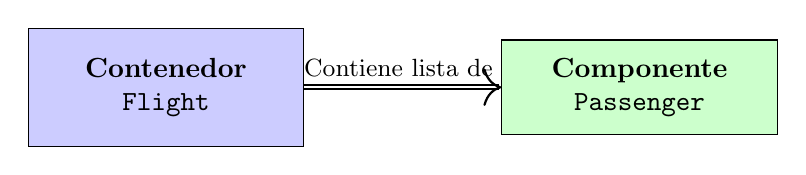
\begin{tikzpicture}[node distance=2cm, align=center]
    \node [draw, rectangle, fill=blue!20, minimum width=3.5cm, minimum height=1.5cm] (vuelo) 
      {\textbf{Contenedor}\\ \texttt{Flight}};
    
    \node [draw, rectangle, fill=green!20, minimum width=3.5cm, minimum height=1.2cm, right=2.5cm of vuelo] (pasajero) 
      {\textbf{Componente}\\ \texttt{Passenger}};
    
    \draw[->, thick, double] (vuelo) -- node[above] {\small Contiene lista de} (pasajero);
  \end{tikzpicture}
  \caption{Relación de Composición: Un Vuelo contiene una lista de Pasajeros.}
  \label{fig:composicion_vuelo}
\end{figure}

A continuación se presenta una clase \texttt{Flight} que gestiona la reserva y capacidad ocupada por objetos \texttt{Passenger}:

\begin{lstlisting}[caption={Ejemplo de Composición con clases Flight y Passenger.}, label={list:composicion_flight}]
class Passenger:
    def __init__(self, name, passport_number):
        self.name = name
        self.passport_number = passport_number

class Flight:
    def __init__(self, flight_number, capacity):
        self.flight_number = flight_number
        self.capacity = capacity
        self.passengers = []  # Lista que almacenara objetos Passenger

    def add_passenger(self, passenger):
        if len(self.passengers) < self.capacity:
            self.passengers.append(passenger)
            print(f"Pasajero {passenger.name} abordado con exito.")
            return True
        else:
            print("Vuelo completo. No se pudo agregar al pasajero.")
            return False

p1 = Passenger("Carlos Gomez", "AB123456")
p2 = Passenger("Maria Lopez", "CD789012")

vuelo = Flight("AR1302", 2)
vuelo.add_passenger(p1)
vuelo.add_passenger(p2)
\end{lstlisting}

Del mismo modo, la composición permite implementar patrones donde una clase administradora procesa de forma polimórfica
una colección de objetos contenidos en su interior:

\begin{lstlisting}[caption={Clase Zoo administrando una colección polimórfica de animales.}, label={list:zoo_animales}]
class Animal:
    def __init__(self, name):
        self.name = name

    def eat(self):
        return f"{self.name} esta comiendo."

class Zoo:
    def __init__(self):
        self.animals = []

    def add_animal(self, animal):
        self.animals.append(animal)

    def feed_all(self):
        for animal in self.animals:
            print(animal.eat())

zoo = Zoo()
zoo.add_animal(Animal("Leon"))
zoo.add_animal(Animal("Panda"))
zoo.feed_all()
\end{lstlisting}


\nocite{*}
\printbibliography

\end{document}
